\documentclass[runningheads]{llncs}
\usepackage{graphicx}
\usepackage[text={150mm,220mm},centering,nohead]{geometry}
\usepackage{listings}

\usepackage{color}
\definecolor{gray}{rgb}{0.4,0.4,0.4}
\definecolor{darkblue}{rgb}{0.0,0.0,0.6}
\definecolor{cyan}{rgb}{0.0,0.6,0.6}

\lstset{
  basicstyle=\ttfamily,
  columns=fullflexible,
  showstringspaces=false,
  commentstyle=\color{gray}\upshape
}
\lstset{breaklines}
\lstdefinelanguage{XML}
{
  morestring=[b]",
  morestring=[s]{>}{<},
  morecomment=[s]{<?}{?>},
  stringstyle=\color{black},
  identifierstyle=\color{darkblue},
  keywordstyle=\color{cyan},
  morekeywords={xmlns,version,type}% list your attributes here
}
\pagestyle{empty}
\begin{document}
\title{\large{CSCI927 Service-Oriented Software Engineering (Progress Report)}}
\author{}
\institute{}
\maketitle
\vspace{-1cm}
%-----------Please Do NOT change the content above.-----------------

%---------------------------------------------------------------------------------------------------------------------------------

%-----------Please write the project information here.---------------

\begin{center}
\Large{\textbf{Online study lounge system based on SOA}} \\ % Please write your project tile in here
\vspace{0.2cm}
\large{\emph{ Liting Lyu (6603324), Yueyue  He (6603671), Muzhe Peng (6603646), Wangzhihui Mei (6603385)}}\\%Please write names of your group members as well as the group number in here
\vspace{0.3cm}
\end{center}

%-----------Please write the content of your research proposal from here.---------------
\noindent %peng muzhe
\section{Progress}
In order to better description the service, the model is further designed according to the proposal. The must-have modules have finished designing, which includes Updates Issue module, Search module and Message Processing Module. The technology of Business Process Modeling Notation(BPMN) and corresponding Extensive Markup Language(XML) are used to denote well-organized and predictable process, Case Management Model and Notation(CMMN) is used to describe the unpredictable process. More details are included in the appendix. 
\\Slight adjustment is made to make the function of the service more appropriate, which is:
\\Deleting the Updates Searching module in the Search service. Because the online study lounge system should focus more on helping users form good habits for study, however it seems unnecessary to search for a certain updates, this module will divert users’ attention more on friends making. 

\section{Next plan}
1.Design the good-to-have services
\\2.Try to apply more technology.
\subsection*{Q\&A Module} %maywzh
\noindent
For Q\&A module, We have developed Question Service and Answer Service along with interaction with Follow Service, Push Service. Down-top design was used to build the system, dividing the application into two layer: basic layer and business logic layer. The SOA pattern was referred in building the System, dividing Question Services and Answer Services into atomic services. BPMN model was used to describe the business process model of the Q\&A module in the view of users. Also, We use CMMN model to describe the case model of the moduel. The according xml files are offered.
Generating Question Services consists search question service, add/edit/follow question services and follow question service, we considered the general business model of the service and combined them into a whold model. In CMMN Model, We connected Question Service and Answer Service, to show the whole service chain.



\clearpage
\begin{flushleft}
    \huge{\textbf{Appendix}}
\end{flushleft}
\begin{center}
    \Large{\textbf{Project Title: Online study lounge system based on SOA }} \\*[0.1cm]%Please write names of the project title in here
    \large{\emph{Group Members (Group number): Liting Lyu (6603324), Yueyue  He (6603671), Muzhe Peng (6603646), Wangzhihui Mei (6603385)}} %Please write names of your group members as well as the group number in here
\end{center}
    %----------------------------------------------------------------------------------------------------------------------------
    
    %-----------Please write the content of your appendix (diagrams, figures, tables, etc) from here.---------------
    %maywzh

	\textbf{Question Service BPMN Model and XML}\\
	\begin{figure}
		\centering %图片居中
		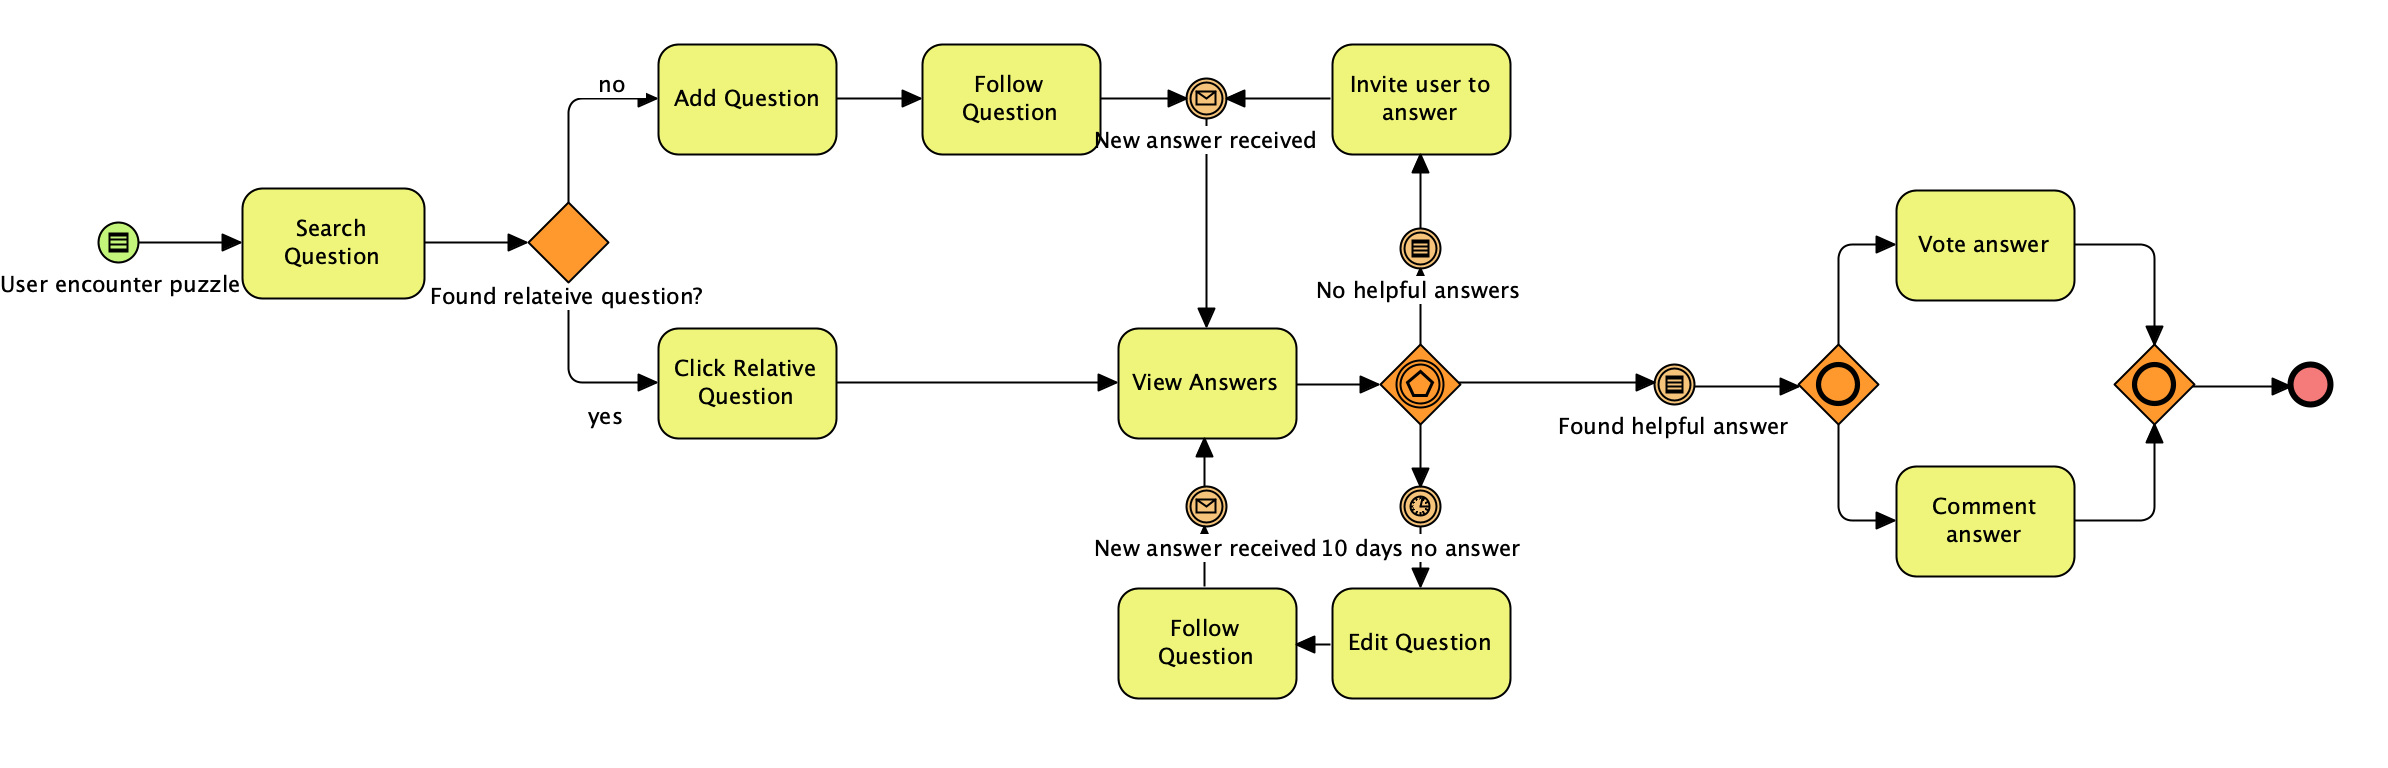
\includegraphics[width=1.0\textwidth]{questionservice} %插入图片,[]中设置图片大小,{}中是图片文件名
		\caption{Question Service} %最终文档中希望显示的图片标题
		\label{questionservice} %用于文内引用的标签
	\end{figure}
    \noindent 
    \begin{lstlisting}[language={XML}]
        <process id="_1" isExecutable="false" name="QuestionService">
		<task completionQuantity="1" id="BP06_BP12" isForCompensation="false" name="Search Question">
			<incoming>BP06_BP22</incoming>
			<outgoing>BP06_BP24</outgoing>
		</task>
		<startEvent id="BP06_BP13" isInterrupting="true" name="User encounter puzzle">
			<outgoing>BP06_BP22</outgoing>
			<conditionalEventDefinition id="ID_14404272_1627_3203_7600_000000200040">
				<condition/>
			</conditionalEventDefinition>
		</startEvent>
		<sequenceFlow id="BP06_BP22" name="" sourceRef="BP06_BP13" targetRef="BP06_BP12"/>
		<exclusiveGateway gatewayDirection="Unspecified" id="BP06_BP23" name="Found relateive question?">
			<incoming>BP06_BP24</incoming>
			<outgoing>BP06_BP29</outgoing>
			<outgoing>BP06_BP30</outgoing>
		</exclusiveGateway>
		<sequenceFlow id="BP06_BP24" name="" sourceRef="BP06_BP12" targetRef="BP06_BP23"/>
		<task completionQuantity="1" id="BP06_BP27" isForCompensation="false" name="Add Question">
			<incoming>BP06_BP29</incoming>
			<outgoing>BP06_BP40</outgoing>
		</task>
		<task completionQuantity="1" id="BP06_BP28" isForCompensation="false" name="Click Relative Question">
			<incoming>BP06_BP30</incoming>
			<outgoing>BP06_BP43</outgoing>
		</task>
		<sequenceFlow id="BP06_BP29" name="no" sourceRef="BP06_BP23" targetRef="BP06_BP27"/>
		<sequenceFlow id="BP06_BP30" name="yes" sourceRef="BP06_BP23" targetRef="BP06_BP28"/>
		<task completionQuantity="1" id="BP06_BP37" isForCompensation="false" name="View Answers">
			<incoming>BP06_BP43</incoming>
			<incoming>BP06_BP44</incoming>
			<incoming>BP06_BP88</incoming>
			<outgoing>BP06_BP71</outgoing>
		</task>
		<task completionQuantity="1" id="BP06_BP39" isForCompensation="false" name="Follow Question">
			<incoming>BP06_BP40</incoming>
			<outgoing>BP06_BP42</outgoing>
		</task>
		<sequenceFlow id="BP06_BP40" name="" sourceRef="BP06_BP27" targetRef="BP06_BP39"/>
		<intermediateCatchEvent id="BP06_BP41" name="New answer received">
			<incoming>BP06_BP42</incoming>
			<incoming>BP06_BP62</incoming>
			<outgoing>BP06_BP44</outgoing>
			<messageEventDefinition id="ID_54404272_1627_3203_7600_000000200041"/>
		</intermediateCatchEvent>
		<sequenceFlow id="BP06_BP42" name="" sourceRef="BP06_BP39" targetRef="BP06_BP41"/>
		<sequenceFlow id="BP06_BP43" name="" sourceRef="BP06_BP28" targetRef="BP06_BP37"/>
		<sequenceFlow id="BP06_BP44" name="" sourceRef="BP06_BP41" targetRef="BP06_BP37"/>
		<endEvent id="BP06_BP45" name="">
			<incoming>BP06_BP69</incoming>
		</endEvent>
		<inclusiveGateway gatewayDirection="Unspecified" id="BP06_BP51" name="Gateway">
			<incoming>BP06_BP73</incoming>
			<outgoing>BP06_BP55</outgoing>
			<outgoing>BP06_BP65</outgoing>
		</inclusiveGateway>
		<task completionQuantity="1" id="BP06_BP53" isForCompensation="false" name="Comment answer">
			<incoming>BP06_BP55</incoming>
			<outgoing>BP06_BP68</outgoing>
		</task>
		<sequenceFlow id="BP06_BP55" name="" sourceRef="BP06_BP51" targetRef="BP06_BP53"/>
		<task completionQuantity="1" id="BP06_BP60" isForCompensation="false" name="Invite user to answer">
			<incoming>BP06_BP77</incoming>
			<outgoing>BP06_BP62</outgoing>
		</task>
		<sequenceFlow id="BP06_BP62" name="" sourceRef="BP06_BP60" targetRef="BP06_BP41"/>
		<task completionQuantity="1" id="BP06_BP64" isForCompensation="false" name="Vote answer">
			<incoming>BP06_BP65</incoming>
			<outgoing>BP06_BP67</outgoing>
		</task>
		<sequenceFlow id="BP06_BP65" name="" sourceRef="BP06_BP51" targetRef="BP06_BP64"/>
		<inclusiveGateway gatewayDirection="Unspecified" id="BP06_BP66" name="Gateway2">
			<incoming>BP06_BP67</incoming>
			<incoming>BP06_BP68</incoming>
			<outgoing>BP06_BP69</outgoing>
		</inclusiveGateway>
		<sequenceFlow id="BP06_BP67" name="" sourceRef="BP06_BP64" targetRef="BP06_BP66"/>
		<sequenceFlow id="BP06_BP68" name="" sourceRef="BP06_BP53" targetRef="BP06_BP66"/>
		<sequenceFlow id="BP06_BP69" name="" sourceRef="BP06_BP66" targetRef="BP06_BP45"/>
		<eventBasedGateway gatewayDirection="Unspecified" id="BP06_BP70" instantiate="false" name="">
			<incoming>BP06_BP71</incoming>
			<outgoing>BP06_BP76</outgoing>
			<outgoing>BP06_BP78</outgoing>
			<outgoing>BP06_BP80</outgoing>
		</eventBasedGateway>
		<sequenceFlow id="BP06_BP71" name="" sourceRef="BP06_BP37" targetRef="BP06_BP70"/>
		<intermediateCatchEvent id="BP06_BP72" name="Found helpful answer">
			<incoming>BP06_BP78</incoming>
			<outgoing>BP06_BP73</outgoing>
			<conditionalEventDefinition id="ID_01527216_1627_3203_7600_000000200061">
				<condition/>
			</conditionalEventDefinition>
		</intermediateCatchEvent>
		<sequenceFlow id="BP06_BP73" name="" sourceRef="BP06_BP72" targetRef="BP06_BP51"/>
		<intermediateCatchEvent id="BP06_BP74" name="No helpful answers">
			<incoming>BP06_BP76</incoming>
			<outgoing>BP06_BP77</outgoing>
			<conditionalEventDefinition id="ID_01527216_1627_3203_7600_000000200062">
				<condition/>
			</conditionalEventDefinition>
		</intermediateCatchEvent>
		<intermediateCatchEvent id="BP06_BP75" name="10 days no answer">
			<incoming>BP06_BP80</incoming>
			<outgoing>BP06_BP82</outgoing>
			<timerEventDefinition id="ID_01527216_1627_3203_7600_000000200063"/>
		</intermediateCatchEvent>
		<sequenceFlow id="BP06_BP76" name="" sourceRef="BP06_BP70" targetRef="BP06_BP74"/>
		<sequenceFlow id="BP06_BP77" name="" sourceRef="BP06_BP74" targetRef="BP06_BP60"/>
		<sequenceFlow id="BP06_BP78" name="" sourceRef="BP06_BP70" targetRef="BP06_BP72"/>
		<sequenceFlow id="BP06_BP80" name="" sourceRef="BP06_BP70" targetRef="BP06_BP75"/>
		<task completionQuantity="1" id="BP06_BP81" isForCompensation="false" name="Edit Question">
			<incoming>BP06_BP82</incoming>
			<outgoing>BP06_BP84</outgoing>
		</task>
		<sequenceFlow id="BP06_BP82" name="" sourceRef="BP06_BP75" targetRef="BP06_BP81"/>
		<task completionQuantity="1" id="BP06_BP83" isForCompensation="false" name="Follow Question">
			<incoming>BP06_BP84</incoming>
			<outgoing>BP06_BP87</outgoing>
		</task>
		<sequenceFlow id="BP06_BP84" name="" sourceRef="BP06_BP81" targetRef="BP06_BP83"/>
		<intermediateCatchEvent id="BP06_BP86" name="New answer received">
			<incoming>BP06_BP87</incoming>
			<outgoing>BP06_BP88</outgoing>
			<messageEventDefinition id="ID_41527216_1627_3203_7600_000000200064"/>
		</intermediateCatchEvent>
		<sequenceFlow id="BP06_BP87" name="" sourceRef="BP06_BP83" targetRef="BP06_BP86"/>
		<sequenceFlow id="BP06_BP88" name="" sourceRef="BP06_BP86" targetRef="BP06_BP37"/>
	</process>
    
	\end{lstlisting}
	\clearpage
	\textbf{Answer Service BPMN Model and XML}\\
	\begin{figure}
		\centering %图片居中
		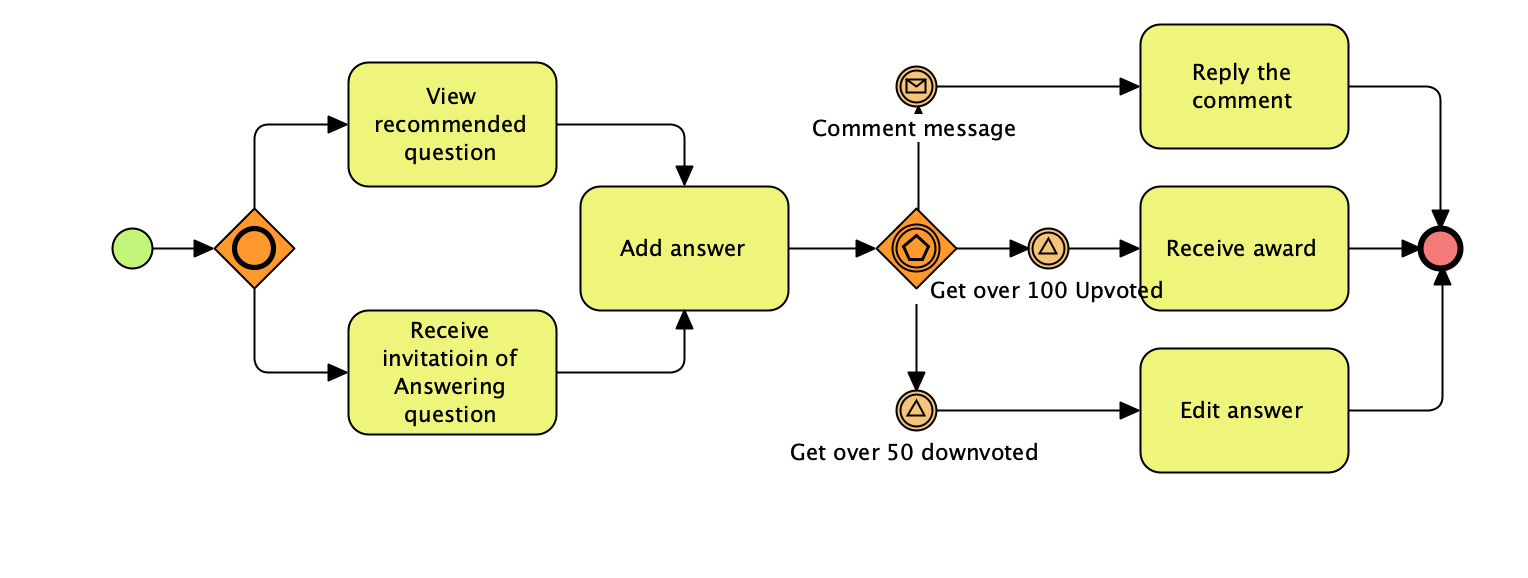
\includegraphics[width=1.0\textwidth]{answerservice} %插入图片,[]中设置图片大小,{}中是图片文件名
		\caption{Answer Service} %最终文档中希望显示的图片标题
		\label{answerservice} %用于文内引用的标签
	\end{figure}
	\begin{lstlisting}[language={XML}]
		<process id="_4" isExecutable="false" name="AnswerService">
		<task completionQuantity="1" id="BP80_BP02" isForCompensation="false" name="View recommended question" startQuantity="1">
			<incoming>BP80_BP27</incoming>
			<outgoing>BP80_BP05</outgoing>
		</task>
		<task completionQuantity="1" id="BP80_BP04" isForCompensation="false" name="Add answer" startQuantity="1">
			<incoming>BP80_BP05</incoming>
			<incoming>BP80_BP29</incoming>
			<outgoing>BP80_BP11</outgoing>
		</task>
		<sequenceFlow id="BP80_BP05" name="" sourceRef="BP80_BP02" targetRef="BP80_BP04" />
		<eventBasedGateway gatewayDirection="Unspecified" id="BP80_BP10" instantiate="false" name="">
			<incoming>BP80_BP11</incoming>
			<outgoing>BP80_BP17</outgoing>
			<outgoing>BP80_BP16</outgoing>
			<outgoing>BP80_BP34</outgoing>
		</eventBasedGateway>
		<sequenceFlow id="BP80_BP11" name="" sourceRef="BP80_BP04" targetRef="BP80_BP10" />
		<task completionQuantity="1" id="BP80_BP12" isForCompensation="false" name="Reply the comment" startQuantity="1">
			<incoming>BP80_BP19</incoming>
			<outgoing>BP80_BP40</outgoing>
		</task>
		<intermediateCatchEvent id="BP80_BP13" name="Comment message">
			<incoming>BP80_BP17</incoming>
			<outgoing>BP80_BP19</outgoing>
			<messageEventDefinition id="ID_47301753_1627_3203_7600_000000200121" />
		</intermediateCatchEvent>
		<sequenceFlow id="BP80_BP17" name="" sourceRef="BP80_BP10" targetRef="BP80_BP13" />
		<sequenceFlow id="BP80_BP19" name="" sourceRef="BP80_BP13" targetRef="BP80_BP12" />
		<task completionQuantity="1" id="BP80_BP23" isForCompensation="false" name="Receive invitatioin of Answering question" startQuantity="1">
			<incoming>BP80_BP28</incoming>
			<outgoing>BP80_BP29</outgoing>
		</task>
		<startEvent id="BP80_BP24" name="">
			<outgoing>BP80_BP26</outgoing>
		</startEvent>
		<inclusiveGateway gatewayDirection="Unspecified" id="BP80_BP25" name="">
			<incoming>BP80_BP26</incoming>
			<outgoing>BP80_BP27</outgoing>
			<outgoing>BP80_BP28</outgoing>
		</inclusiveGateway>
		<sequenceFlow id="BP80_BP26" name="" sourceRef="BP80_BP24" targetRef="BP80_BP25" />
		<sequenceFlow id="BP80_BP27" name="" sourceRef="BP80_BP25" targetRef="BP80_BP02" />
		<sequenceFlow id="BP80_BP28" name="" sourceRef="BP80_BP25" targetRef="BP80_BP23" />
		<sequenceFlow id="BP80_BP29" name="" sourceRef="BP80_BP23" targetRef="BP80_BP04" />
		<sequenceFlow id="BP80_BP16" name="" sourceRef="BP80_BP10" targetRef="BP80_BP14" />
		<intermediateCatchEvent id="BP80_BP14" name="Get over 100 Upvoted">
			<incoming>BP80_BP16</incoming>
			<outgoing>BP80_BP32</outgoing>
			<signalEventDefinition id="ID_27301753_1627_3203_7600_000000200122" />
		</intermediateCatchEvent>
		<task completionQuantity="1" id="BP80_BP31" isForCompensation="false" name="Receive award" startQuantity="1">
			<incoming>BP80_BP32</incoming>
			<outgoing>BP80_BP41</outgoing>
		</task>
		<sequenceFlow id="BP80_BP32" name="" sourceRef="BP80_BP14" targetRef="BP80_BP31" />
		<intermediateCatchEvent id="BP80_BP33" name="Get over 50 downvoted">
			<incoming>BP80_BP34</incoming>
			<outgoing>BP80_BP36</outgoing>
			<signalEventDefinition id="ID_27301753_1627_3203_7600_000000200123" />
		</intermediateCatchEvent>
		<sequenceFlow id="BP80_BP34" name="" sourceRef="BP80_BP10" targetRef="BP80_BP33" />
		<task completionQuantity="1" id="BP80_BP35" isForCompensation="false" name="Edit answer" startQuantity="1">
			<incoming>BP80_BP36</incoming>
			<outgoing>BP80_BP42</outgoing>
		</task>
		<sequenceFlow id="BP80_BP36" name="" sourceRef="BP80_BP33" targetRef="BP80_BP35" />
		<endEvent id="BP80_BP37" name="">
			<incoming>BP80_BP40</incoming>
			<incoming>BP80_BP41</incoming>
			<incoming>BP80_BP42</incoming>
		</endEvent>
		<sequenceFlow id="BP80_BP40" name="" sourceRef="BP80_BP12" targetRef="BP80_BP37" />
		<sequenceFlow id="BP80_BP41" name="" sourceRef="BP80_BP31" targetRef="BP80_BP37" />
		<sequenceFlow id="BP80_BP42" name="" sourceRef="BP80_BP35" targetRef="BP80_BP37" />
	</process>
	\end{lstlisting}

	\textbf{Q\&A Service CMMN Model and XML}\\
	\begin{figure}
		\centering %图片居中
		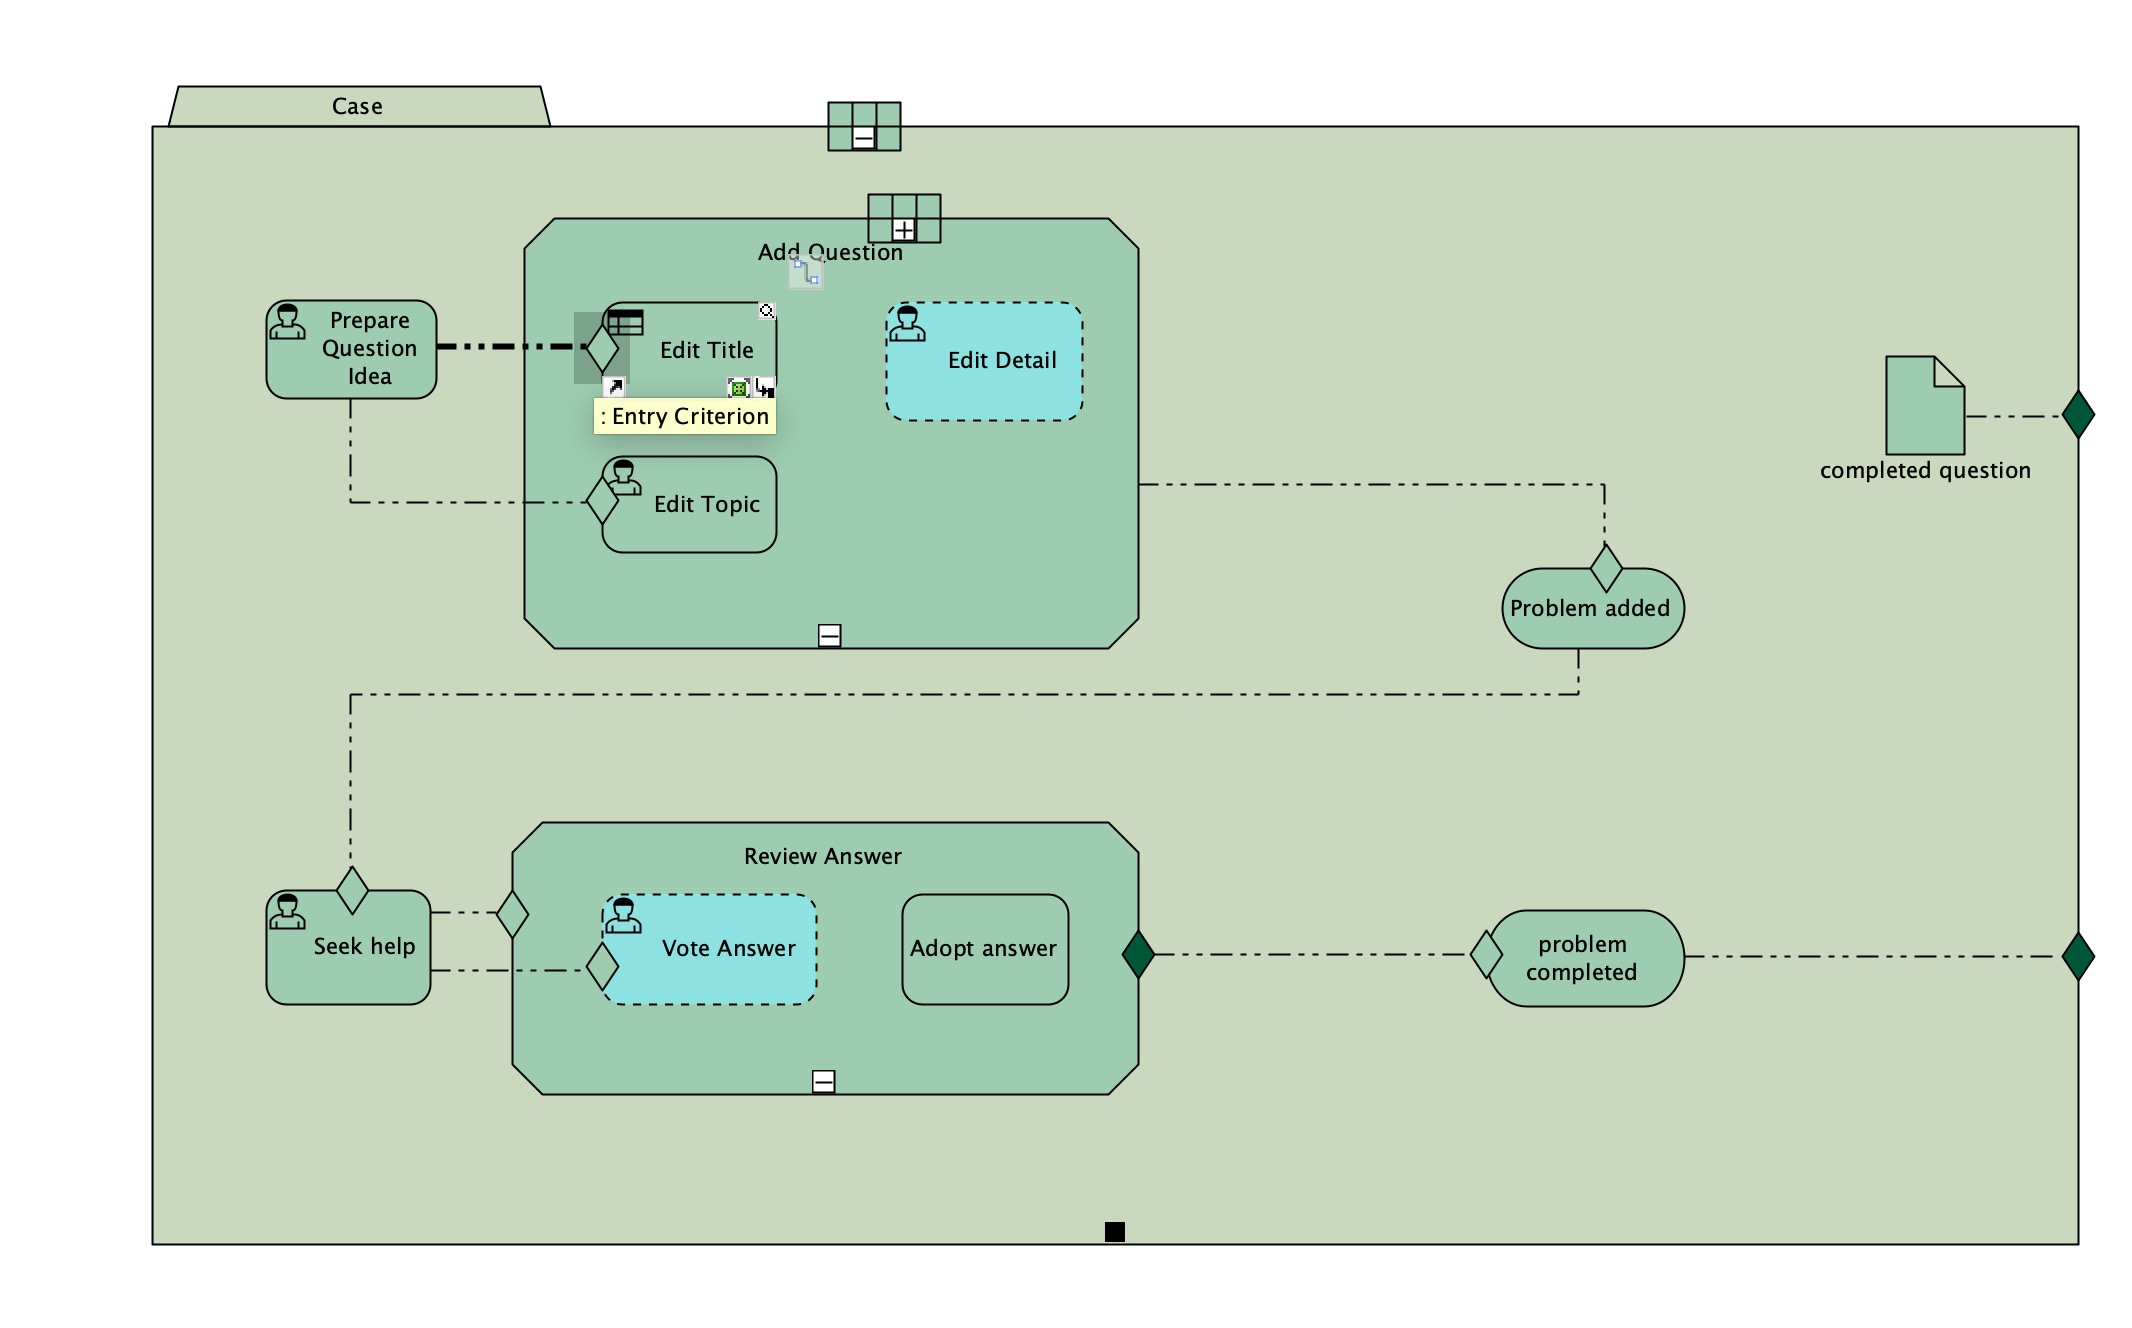
\includegraphics[width=1.0\textwidth]{cmmnmodel} %插入图片,[]中设置图片大小,{}中是图片文件名
		\caption{Q\&A Service CMMN Model} %最终文档中希望显示的图片标题
		\label{qaservice} %用于文内引用的标签
    \end{figure}   
    
    %pengmuzhe
    
    %heyueyue
    
    %lvliting

	\clearpage

\end{document}
